\chapter{总体设计}

本章围绕“基于移动平台的固定目标识别及瞄准系统”给出总体方案，重点说明系统工作原理、模块关系与性能约束，为后续器件选型、硬件实现与软件设计提供统一依据。

\section{系统设计工作原理及原理框图}

\subsection{基本工作原理}

系统以“视觉感知 + 惯性测量 + 双闭环控制”为核心链路：摄像头完成目标图像采集与误差提取，IMU提供高频角速度信息，控制器根据像素偏差与角速度前馈生成云台控制量，实现对固定目标的持续指向与误差抑制。

在执行过程中，系统按照“采集-估计-控制-反馈”循环运行。外环以像素误差为主，内环以角速度补偿为主，从而兼顾稳态精度与动态响应。
从计算节点角度看，系统由三个协同工作的处理单元构成：

（1）\textbf{Linux视觉节点}：以通用计算平台运行OpenCV视觉管线，完成目标检测、位姿解算与跟踪状态管理，结果通过串口协议下发给云台主控；

（2）\textbf{云台主控节点（STM32H7）}：以480\,MHz主频实时处理IMU数据、执行双轴伺服控制和瞄准解算，并通过RS485总线驱动MS4010双轴电机；

（3）\textbf{底盘主控节点（独立单片机）}：独立执行八路灰度传感器循迹、编码器PI速度闭环与圈次任务，与云台节点通过接口协同而非控制耦合，互不干扰。

该三节点架构将视觉计算、姿态控制和底盘机动分散到各自最适合的平台，降低单节点负担的同时提升系统可扩展性。
\subsection{系统原理框图与模块说明}

系统总体由移动底盘、云台执行机构、视觉采集模块、IMU模块、主控与通信模块、上位机监控模块构成。各模块间通过标准接口进行数据交互，形成可扩展、可维护的分层结构。系统总体框图如图\ref{fig:system-overview}所示。

\begin{figure}[htbp]
\centering
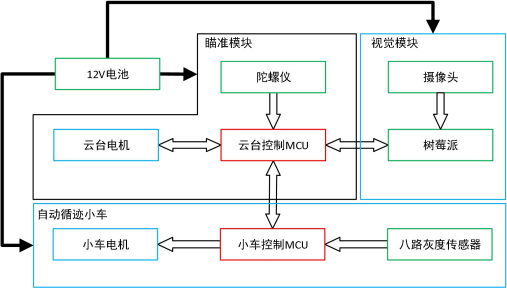
\includegraphics[width=0.85\textwidth]{images/chapters/fig-system-overview.png}
\caption{系统总体框图}
\label{fig:system-overview}
\end{figure}

如图所示，系统分为三个功能子系统：瞄准模块（STM32H7云台控制MCU + 陀螺仪 + 云台电机）、视觉模块（摄像头 + 树莓派/Linux视觉节点）以及自动循迹小车（小车控制MCU + 八路灰度传感器 + 小车电机）。各子系统通过串口/RS485互联，以12\,V电源总线统一供电。

其中，主控侧负责实时控制与状态发布；上位机侧负责参数配置、可视化监测与实验数据记录。该分层架构便于后续算法替换与功能迭代。

在节点间通信层面，各链路数据类型与协议各异：Linux视觉节点以固定帧格式\texttt{@px,py,flag,\#}通过串口向云台主控输出目标像素坐标与置信标志；云台主控通过RS485总线与MS4010电机通信，完成角度指令打包、响应解析与超时检测；底盘主控以独立控制器实现内部闭环，与上层通过预定义接口完成模式同步。这种"链路分离"设计使各子系统在对方降级时仍能维持最小功能闭环，提升了整体鲁棒性。

\section{系统设计要求}

\subsection{功能性要求}

系统应具备目标识别与连续跟踪、云台姿态控制、实时状态回传、参数在线整定等基础功能。核心任务是在移动平台运动扰动下保持瞄准线稳定。

\subsection{性能指标要求}

结合开题目标，系统设计以低成本平台为约束，重点满足以下定量指标，如表\ref{tab:performance_requirements}所示。

\begin{table}[htbp]
\centering
\begin{tabular}{llll}
\hline
指标类别 & 指标项 & 设计目标 & 说明 \\
\hline
视觉实时性 & 视觉帧率 & $\geq$25\,FPS & 室内标准光照场景 \\
惯性采样 & IMU采样频率 & $\geq$100\,Hz & 角速度前馈需求 \\
瞄准精度 & 稳态指向误差 & $\leq$0.8\,mrad & 静态目标双闭环收敛后 \\
成本约束 & 整机器件成本 & 千元级（$\leq$\yen{}1000） & 不含通用计算平台 \\
功耗约束 & 系统功耗 & $\leq$5\,W & 嵌入式部分 \\
重量约束 & 嵌入式系统重量 & $\leq$500\,g & 含云台机构 \\
\hline
\end{tabular}
\caption{系统性能指标要求}
\label{tab:performance_requirements}
\end{table}

其中，0.8\,mrad的稳态误差指标来源于对典型室内应用场景的分析；25\,FPS视觉帧率保证像素闭环具备足够带宽裕量；100\,Hz IMU采样频率则确保前馈补偿对平台机动具有及时响应能力。

\subsection{约束条件与设计边界}

系统设计受限于本科毕设条件与嵌入式算力，遵循“低成本、低功耗、可复现”的工程边界，不依赖高功耗GPU与昂贵传感器。在此约束下，优先选择成熟、易调试、易复现的实现路线。

\section{关键器件选型与接口设计}

为落实总体设计目标，本节在“可获取性、接口兼容性、实时性、工程可复现性”原则下完成关键器件选型与接口关系定义，使系统方案从架构层进一步落到可实现的工程层。

\subsection{主控器件}

云台控制系统需要处理来自IMU和视觉模块的多源数据，并在实时控制周期内完成角速度前馈补偿与伺服控制的计算。因此主控器件必须具备较高的主频、充足的存储资源和完善的外设接口，同时需要支持定时控制、中断管理和通信协议扩展，并具有健全的开发生态以便快速开发。

结合这些需求，本课题选用STM32H7系列微控制器作为云台主控平台。其中STM32H743XIH6的CPU主频高达480\,MHz，内置单精度与双精度浮点运算单元（FPU）及DSP指令集，能够承担IMU数据处理、控制律计算与通信管理等高实时性任务。同时STM32H7生态成熟，支持移植RT-Thread实时操作系统，便于快速调用各类驱动资源进行高效开发。相较于其他微控制器方案（如MSPM0G3507主频仅80\,MHz），STM32H7在计算能力和浮点性能上具有显著优势，更能满足云台双轴伺服、IMU前馈补偿与视觉数据融合需要同频运行的实时控制需求。

\subsection{传感器与视觉模块}

系统采用六轴惯性测量单元（IMU）用于姿态感知与角速度前馈，其输出数据为动态补偿提供了高频的输入信息，能够在平台运动状态下有效提升瞄准稳定性。经过零偏校准与滤波处理后，惯性传感器的测量精度可以进一步提高。选取IMU时需要确保角速度测量稳定、采样频率可灵活配置、通信接口可靠且抗干扰能力强，同时与主控平台在通信协议和电气特性上兼容。

在视觉模块方面，课题采用USB摄像头作为图像输入源。与专用视觉芯片模块（如MaixCAM等）相比，USB摄像头的部署成本低、驱动生态完善，便于与上位机图像处理流程集成。更重要的是，USB摄像头配合Linux平台能够直接运行OpenCV传统视觉算法，在本课题以HSV色彩分割和PnP位姿解算为核心的目标识别链中，帧率表现稳定且一致性好。此外，摄像头体积小、重量轻，易于架设在云台机构上随动，符合轻量化的系统设计目标。

\subsection{执行机构与接口设计}

云台的执行机构需要具备快速响应、精度可调、驱动稳定和维护简便等特点，并须与主控的输出信号相互匹配。在电机方案选择中，本课题对比了两种技术路线：其一为张大头自闭环步进电机云台，具有精度高、通讯简单的优点，但两轴步进电机组合后机械体积偏大，不利于整机的轻量化设计；其二为采用RS485接口的小型无刷云台机构，在满足控制精度要求的同时具备更为紧凑的体积和更轻的重量，与STM32H7的输出信号具有良好的兼容性。综合结构、性能等多方面因素，选择方案二作为执行机构。通过合理的驱动电路设计与闭环控制策略，可实现方位与俯仰通道的协调控制。

系统的信号连接采用RS485总线串口通讯方式。STM32H743通过UART外设与RS485收发器相连，按照MS4010协议向偏航轴（ID\,1）和俯仰轴（ID\,2）的电机发送速度或位置指令帧。相比于PWM驱动方案，RS485总线具有更强的抗干扰能力和多节点扩展潜力，通信速率可达1\,Mbit/s，足以满足500\,Hz的控制周期实时要求。清晰的接口定义规范有利于后续系统联调复杂度的降低。

同时，本系统充分利用STM32H7的丰富外设资源：串口用于与RS485模块和通信设备通讯，定时器负责周期性的控制任务调度，PWM模块驱动执行器，而I2C或SPI接口用于传感器数据采集。IMU与主控通过标准数字接口完成数据交互，摄像头则与上位机侧构成独立的图像采集链路。两路数据流在控制层按时间顺序进行融合处理，保证控制计算的时间一致性和数据同步性。

\section{本章小结}

本章围绕总体设计主线，完成了系统工作机理、三节点分布式架构设计、定量性能指标约束以及关键器件选型与接口关系定义，形成了从"方案定义"到"工程落地"的完整闭环，为下一章硬件详细设计与实现提供了直接依据。
